\section{EC 3.14}
\textbf{Exercise 14.0.1} (Market model definition). \textit{Provide the definition of the market model used by Arrow and Debreu.}\\

Consider a market model as follows:
\begin{itemize}
\item $N=\{1, \ldots, n\}$ is the set of players;
\item $K=\{1, \ldots, k\}$ is the set of perfectly divisible commodities;
\item $x_{i} \in \mathbb{R}_{+}^{k}$ with $i \in N$ is a vector of $k$ elements, where $x_{i, j},$ denoting the element in the $j$-th position of the vector, represents the amount of commodity $j$ available to player $i$;
\item $e_{i} \in \mathbb{R}_{+}^{k}$ with $i \in N$ is the initial endowment of player $i$ and $e_{i, j}$ is the initial endowment for commodity $j$;
\item $u_{i}: \mathbb{R}_{+}^{k} \rightarrow \mathbb{R}_{+}$ is the utility function of player $i$ that is continuous and concave;
\item $p \in \mathbb{R}_{+}^{k}$ is a vector of $k$ elements, where $p_{j},$ denoting the element in the $j$-th position of the vector, represents the price of commodity $j$.
\end{itemize}
Each player maximizes her utility function under budget constraints by buying/selling commodities. Formally, we have:
\[
\begin{array}{cl}
\max _{x_{i}} & u_{i}\left(x_{i}\right) \\
\text { s.t. } & p \cdot x_{i} \leqslant p \cdot e_{i}
\end{array}
\]
where $p \cdot e_{i}$ represents the budget available to player $i,$ while the argument of the above optimization problem, denoted by $x_{i}^{*},$ is the best amount of commodity for player $i$ given the market prices and the budget constraints. Notice that the above optimization problem does not take into account any constraint related to the amount of commodities available in the market. Thus, in principle, the above optimization problem may return a $x_{i}^{*}$ that is not implementable in practice, requiring an excessive amount of commodities larger than that one actually available in the market.\\

\textbf{Exercise 14.0.2} (Market clearing). \textit{Provide the definition of market clearing.}\\

The market clears when the total amount of commodities $x=\sum_{i \in N} x_{i}$ equals to total amount of initial endowments $e=\sum_{i \in N} e_{i}$.\\
Notice that, when the price vector is arbitrary, there is no guarantee that the market clears. For instance, as already mentioned above, it may happen that the vector $x$ is larger than $e$ for some commodities. The market clearing property is of paramount importance and depends on the price vector. Indeed, when this property holds, each player in the market acts independently from the others. In other words, each player negotiates with a fictitious player corresponding to the market. This allows one to neglect the direct interaction between the players when searching for the market outcome.

Thus, the study of the conditions under which the market clears is crucial. This is stated by the Arrow-Debreu theorem.\\

\textbf{Exercise 14.0.3} (Arrow-Debreu equilibrium). \textit{Provide the definition of the Arrow-Debreu equilibrium and argue the meaning of the result.}\\

There is always a price vector $p^{*}$ such that $\sum_{i \in N} x_{i}^{*} \leqslant e$ and $p^{*}$ is Pareto efficient for the players.\\
The problem of finding an Arrow-Debreu equilibrium is slightly different from the problem of finding a Nash equilibrium. On the one hand, each player behaves rationally, maximizing her utility function, asin a Nash equilibrium. In particular, the problem reduces to the problem of finding a Nash equilibrium when prices are fixed. On the other hand, prices are part of the problem. Thus the problem of finding an Arrow-Debreu equilibrium can be formulated as the problem of finding prices satisfying some conditions under the equilibrium constraints of the players.Interestingly, the problem of finding an Arrow-Debreu equilibrium presents the same computational properties of the problem of finding the Nash equilibrium, as stated below.

\section{EC 3.15}
\textbf{Exercise 15.0.1} (Leader-Follower equilibrium definition). \textit{Provide the definition of the Leader-Follower equilibrium with 2 players.}\\

The problem of finding a Leader–Follower equilibrium is formulated as:
\begin{figure}[H]
\centering
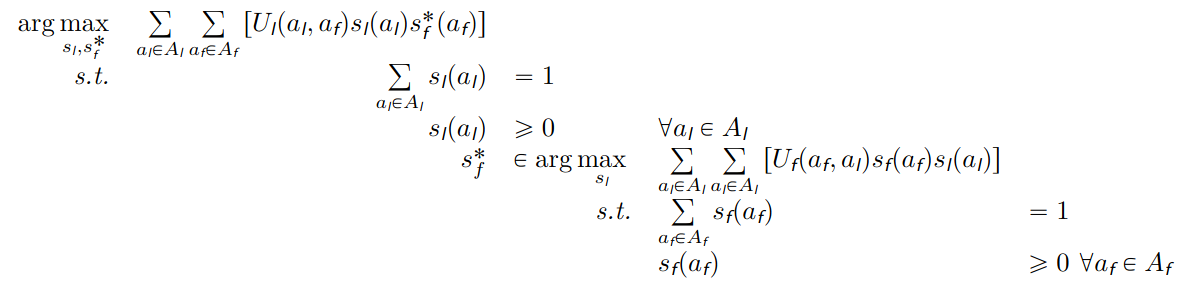
\includegraphics[width=\textwidth]{images/img_3_15_01.png}
\end{figure}

\textbf{Exercise 15.0.2} (Leader-Follower equilibrium properties). \textit{Describe the properties of the Leader-Follower equilibrium with 2 players.}\\

\textbf{Exercise 15.0.3} (Leader-Follower equilibrium example). \textit{Given a 2-player normal-form game with 2 actions per player, find a Leader-Follower equilibrium.}\\

\textbf{Exercise 15.0.4} (Leader-Follower equilibrium formulation). \textit{Provide the mathematical programming formulation to find a Leader-Follower equilibrium with 2 players.}\\

\textbf{Exercise 15.0.5} (Finding a Leader-Follower equilibrium). \textit{Given a 2-player normal-form game, find a Leader-Follower equilibrium by means of AMPL+GUROBI.}\\

\textbf{Exercise 15.0.6} (Leader-Follower equilibrium complexity). \textit{What is the computational complexity of finding a Leader-Follower equilibrium?}\\

\textbf{Exercise 15.0.7} (Leader-Follower equilibrium vs.  Nash equilibrium). \textit{Describe the relationships between Leader-Follower equilibrium and Nash equilibrium.}\\

\textbf{Exercise 15.0.8} (Leader-Follower equilibrium formulation with multi-type follower). \textit{Provide the mathematical programming formulation to find a Leader-Follower equilibrium with 2 players when the follower can be of multiple types.}\\

\textbf{Exercise 15.0.9} (Finding a Leader-Follower equilibrium). \textit{Given a 2-player normal-form game in which the follower can be of multiple types, find a Leader-Follower equilibrium by means of AMPL+GUROBI.}\\

\textbf{Exercise 15.0.10} (Leader-Follower equilibrium complexity). \textit{What is the computational complexity of finding a Leader-Follower equilibrium when the follower can be of multiple types?}\\

\section{EC 3.16}

\textbf{Exercise 16.0.1} (Congestion game definition). \textit{Provide the definition of Congestion game.}\\

\textbf{Exercise 16.0.2} (Pure-strategy Nash equilibrium in congestion games). \textit{Prove that every finite congestion game admits at least a pure-strategy Nash equilibrium.}\\

\textbf{Exercise 16.0.3} (Best-response paths). \textit{Provide the definition of best-response paths and prove that in every finite congestion game all the best-response paths are finite.}\\

\textbf{Exercise 16.0.4} (Finding best-response paths). \textit{Given a congestion game, find a best-response path.}\\

\textbf{Exercise 16.0.5} (Potential functions). \textit{Provide the definitions of potential functions and discuss the relation-ships between potential games and congestion games.}\\

\textbf{Exercise 16.0.6} (Characterization of games admitting an exact potential function). \textit{Discuss when a normal-form game admits an exact potential function and prove that.}\\

\textbf{Exercise 16.0.7} (Inefficiency bounds). \textit{Provide the definition of Price of Anarchy and Price of Stability.}\\

\textbf{Exercise 16.0.8} (PoA and PoS unboundness). \textit{Provide an example in which PoA and PoS are unbounded.}\\

\textbf{Exercise 16.0.9} (Upper bound over best-response paths length). \textit{Provide an upper bound over the length of best-response paths in singleton congestion games and prove it.}

\section{EC 3.17}
\textbf{Exercise 17.0.1} (Social choice functions). \textit{Provide the definition of social choice function. Provide one example.}\\

\textbf{Exercise 17.0.2} (Efficiency). \textit{Provide the definitions of ex ante, ex interim, ex post efficiency for social choice functions. Answer to the following questions.
\begin{itemize}
\item Is the social choice function implemented by the Second-Price auction efficient in ex post?
\item Provide an example of social choice function that is efficient in ex post, but not in ex interim.
\item Provide an example of social choice function that is efficient in ex interim, but not in ex post.\\
\end{itemize}}

\textbf{Exercise 17.0.3} (Individual rationality). \textit{Provide the definitions of ex ante, ex interim, ex post individual rationality for social choice functions. Answer to the following questions.
\begin{itemize}
\item Is the social choice function implemented by the Second-Price auction individually rational in ex post?
\item Provide an example of social choice function that is individually rational in ex interim, but not in ex post.
\item Provide an example of social choice function that is individually rational in ex ante, but not in ex interim.
\item Provide an example of social choice function that is individually rational in ex interim, but not in ex ante.\\
\end{itemize}}

\textbf{Exercise 17.0.4} (Dictatorship). \textit{Provide the definition of dictatorship for social choice functions. Provide an example.}\\

\section{EC 3.18}

\textbf{Exercise 18.0.1} (Economic mechanism). \textit{Provide the definition of economic mechanism.}\\

\textbf{Exercise 18.0.2} (Implementation of a social choice function). \textit{Provide the definition of implementation of asocial choice function.}\\

\textbf{Exercise 18.0.3} (Direct-revelation mechanism). \textit{Provide the definitions of direct-revelation mechanism and indirect-revelation mechanism and provide an example for each one of them.}\\

\textbf{Exercise 18.0.4} (Incentive compatibility). \textit{Provide the definition of incentive compatibility.}\\

\textbf{Exercise 18.0.5} (Checking incentive compatibility). \textit{Given a social choice function, check whether it is incentive compatible.}\\

\textbf{Exercise 18.0.6} (Revelation principle for Dominant-Strategy equilibrium). \textit{Provide the statement of the rev-elation principle and the proof.}\\

\textbf{Exercise 18.0.7} (Gibbard-Satterthwaite impossibility theorem). \textit{Provide the statement of the Gibbard-Satterthwaite impossibility theorem.}\\